\subsection{Unveiling the Third Circle: Enhancing Smith Chart Design!}

\begin{tcolorbox}[colback=gray!10, colframe=black, title=E9G09] What third family of circles is often added to a Smith chart during the process of designing impedance matching networks?
\begin{enumerate}[label=\Alph*.]
    \item \textbf{Constant-SWR circles}
    \item Transmission line length circles
    \item Coaxial-length circles
    \item Radiation-pattern circles
\end{enumerate} \end{tcolorbox}

\subsubsection{Explanation of Concepts}

The Smith chart is a powerful graphical tool used in radio frequency (RF) engineering for visualizing complex impedance and reflection coefficients. It aids engineers in designing impedance matching networks, which are crucial for maximizing power transfer and minimizing signal loss in communication systems.

\subsubsection*{Constant-SWR Circles:}
Constant standing wave ratio (SWR) circles represent points of equal SWR on the Smith chart. As SWR is a measure of the efficiency of power transfer, these circles are critical for evaluating how well a load is matched to a transmission line. The use of constant-SWR circles helps engineers determine where to place components such as capacitors and inductors to achieve optimal matching.

\subsubsection*{Other Circle Families:}
- \textbf{Transmission line length circles:}: These circles represent points of equal electrical length of the transmission line.
- \textbf{Coaxial-length circles:}: These are generally not used in conjunction with a Smith chart.
- \textbf{Radiation-pattern circles:}: These pertain to the directivity of antennas rather than impedance.

\subsubsection*{Calculation Steps:}
To properly utilize the Smith chart:
1. Start by plotting the normalized impedance on the Smith chart.
2. Identify the corresponding SWR circles; these will guide you in creating a matching network.
3. Use the intersection of your load impedance and SWR circles to determine the required reactive components.

\subsubsection{Diagram}
Below is a simple representation of the Smith chart with indicated constant-SWR circles.

\begin{center}
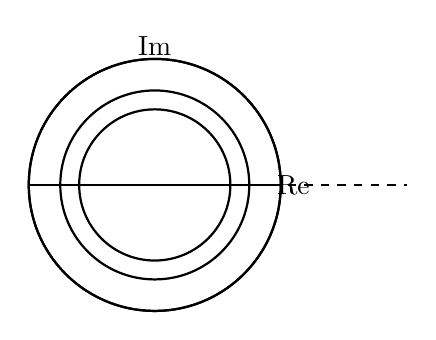
\begin{tikzpicture}[scale=0.8]
    % Draw the outer circle (unit circle)
    \draw[thick] (0,0) circle (2);
    % Draw the real axis
    \draw[thick] (-2,0) -- (2,0);
    % Draw constant SWR circles
    \foreach \r in {1.2, 1.5, 2.0} {
        \draw[thick,dashed] (0,0) -- (\r*2,0);
        \draw[thick] (0,0) circle (\r);
    }
    % Label the axes
    \node at (2.2,0) {Re};
    \node at (0,2.2) {Im};
    % Note: Add appropriate SWR and matching labels as needed
\end{tikzpicture}
\end{center}

The constant-SWR circles on the Smith chart illustrate how impedance matching networks can be designed by observing the intersection points with the load impedance and adjusting the network accordingly. Proper use of this tool enables efficient design in RF applications.
